\documentclass[11pt,oneside]{book}
\usepackage[margin=1.2in]{geometry}
\usepackage[toc,page]{appendix}
\usepackage{graphicx}
\usepackage{longtable}
\usepackage{natbib}
\usepackage{lipsum}
\usepackage{caption}
\usepackage{multicol}
\usepackage{csquotes}

\begin{document}

\captionsetup[figure]{margin=1.5cm,font=small,labelfont={bf},name={Figure},labelsep=colon,textfont={it}}
\captionsetup[table]{margin=1.5cm,font=small,labelfont={bf},name={Table},labelsep=colon,textfont={it}}
\setlipsumdefault{1}

\frontmatter

\begin{titlepage}


% -------------------------------------------------------------------
% You need to edit the details here
% -------------------------------------------------------------------

\begin{center}
{\LARGE University of Sheffield}\\[1.5cm]
\linespread{1.2}\huge {\bfseries Size Matters: Acquiring Vague Spatial Size Information from Textual Sources}\\[1.5cm]
\linespread{1}

\includegraphics[width=5cm]{images/tuoslogo.png}\\[1cm]
{\Large Alexander White}\\[1cm]
{\large \emph{Supervisor:} Dr Robert Gaizauskas}\\[1cm]
\large A report submitted in partial fulfilment of the requirements\\ for the degree of Computer Science with a Year in Industry BSc in Computer Science\\[0.3cm] 
\textit{in the}\\[0.3cm]
Department of Computer Science\\[2cm]
\today
\end{center}

\end{titlepage}


% -------------------------------------------------------------------
% Declaration
% -------------------------------------------------------------------

\newpage
\section*{\Large Declaration}

All sentences or passages quoted in this document from other people's work have been specifically acknowledged by clear cross-referencing to author, work and page(s).  Any illustrations that are not the work of the author of this report have been used with the explicit permission of the originator and are specifically acknowledged.  I understand that failure to do this amounts to plagiarism and will be considered grounds for failure.\\[1cm]

\noindent Name: Alexander White\\[1mm]
\rule[1em]{25em}{0.5pt}

\noindent Signature:\\[1mm]
\rule[1em]{25em}{0.5pt}

\noindent Date:\\[1mm]
\rule[1em]{25em}{0.5pt}


% -------------------------------------------------------------------
% Abstract
% -------------------------------------------------------------------

\chapter*{\Large \center Abstract}

Size estimation of an object is a task that humans can perform easily but struggle to explain the process of. It is common sense to be able to estimate the size of an object. This dissertation project aims to create a database of objects with their commonly found sizes to assist software in being able to make these same estimates. The project will achieve this by using information extraction techniques to find written examples of object's sizes. The final system will use named entity recognition and relationship extraction to obtain this information from a text source.

% -------------------------------------------------------------------
% Contents, list of figures, list of tables
% -------------------------------------------------------------------

\tableofcontents
\listoffigures
\listoftables


% -------------------------------------------------------------------
% Main sections (as required)
% -------------------------------------------------------------------

\mainmatter

\chapter{Introduction}

Understanding an object's size can help machine learning models in image and video recognition by allowing estimation of an unknown object's size by comparing it with other objects in the image. For example, if you had to classify an object in an image as either a dog or a horse knowing that it was standing next to a person, and that on average a person is larger than a dog but smaller than a horse, this could inform your classification.

This dissertation takes on the problem of determining the general sizes of different objects. Humans are talented at estimating sizes of objects based on common sense or memory. This can help us make estimations about new objects, judge the distance of an object, or to generate accurate simulated landscapes.

Named entity recognition techniques have been shown to produce accurate results, as have relationship extraction models. Combining this with gazetteers for objects or units of size is likely to give good results. The limitation to these models will be the quality and quantity of the training data. This is a trade-off, increasing the quality of our data takes more time and therefore reduces the quantity we can gather. Therefore, this project will go with a semi-supervised learning technique that tries to strike a good balance between the two.

\section{Aims and Objectives}

The aim of this dissertation is to make progress towards creating a database containing information about objects and their usual sizes. This can be broken down into three stages. Stage one is fulfilling our requirement to acquire data containing various objects and sizes. The aim is to train machine learning models to be able to identify objects and sizes within a sentence and determine if they are related. To collect enough data to adequately train these models we will use semi-supervised learning, which means that this stage will run simultaneously alongside stage two.

Stage two is building the named entity recognition and relationship extraction models for both identifying objects and sizes in text and determining if they are related. To help with the semi-supervised learning we can build some very basic models to start collecting data. Using regular expressions to determine sizes, and part-of-speech tagging to determine nouns, we can build models with poor accuracy but that will help in collecting data that can be refined into the final training set. This final training set will be used to train the models and from there we can refine them to get the most accurate results.

The final stage of the project will be to collect all the results into a database. The accuracy of the collected data can be improved if objects have been found multiple times. We can look at previously found sizes of the object to determine if this new measurement is accurate. If we introduce an object hierarchy to determine if objects are related, then we can also use similar objects to estimate realistic sizes.

Examples of the sort of sentences we will be trying to identify and extract information from:
\begin{displayquote}
“Mountains are usually at least 500m tall."
\\“My house is 500m from the closest shop."
\\“The average apple is 6cm (2 inches) in diameter."
\end{displayquote}

\noindent In the first sentence there is one object, one size, and they are related. In the second sentence there are two objects and one size, none of which are related, and in the third there is one object and two sizes, both which describe the object. It becomes apparent very quickly the variety in which objects can be described and this is going to be the challenge in fulfilling the aims of this project.

\section{Overview of the Report}

This report will begin with a literature survey, explaining the different options and previously tried techniques for various problems this project will face. It will give an overview of the techniques, their advantages, and disadvantages.

This will be followed by an in-depth investigation into the requirements of the project and an analysis of the problem and how the project will be tackling it. This will be similar to the literature survey except it will only discuss why a technique has been chosen over another with regards to the nature of the project.

This will be followed by explaining the design and implementation of the techniques used in this project, as well as how the results were obtained and what tests were run.

Finally, there will be a discussion and conclusion about the projects aims and final results.


\chapter{Literature Survey}

There has not been much previous work done on this topic, but each of the individual aspects of the project has been researched in depth by other parties. The majority of the project is an information extraction task which has been widely researched with many techniques to perform well on various forms of data. Other considerations to be made will be what tools or programming languages to use, and how to store both the training data and the results.

\section{Information Extraction}
The information extraction task can be broken down into two parts, named entity recognition and relationship extraction. The difference in these two tasks would be indentifying the objects and sizes within the sentence, and then determining if they are related. For example, with the sentence “Beech trees can grow to more than 40m.”, named entity recognition is the task of identifying “Beech trees” as an object and “40m” as a size. Relationship extraction is the task of determining whether the size is a description of the object i.e. whether they are related. This section will overview the problem, different techniques for the tasks, their advantages, and their disadvantages.

\subsection{Named Entity Recognition}

Named entity recognition is the process of identifying entities in text. This task can be broken down into finding the entities and classifying them into classes. The most common classes used for named entities are person names, organisations, and locations but you can build models to identify any class of entity. There are many challenges that come along with this, such as coreference, which is when an entity is referred to in the text but not by name. For example: “Henry Ford was born in 1863. He is known for founding the Ford Motor Company.”. In the second sentence the entity “Henry Ford” is referred to as “He”. This is called coreference and needs to be resolved before entities can be identified if you want to capture all occurrences of the entities.

Three primary approaches to named entity recognition are knowledge-engineering, supervised learning, and semi-supervised learning \citep{text_processing_lecture_5}:

\subsubsection{Knowledge-Engineering}

Knowledge-engineering approaches use gazetteers and human written rules to determine if a token is an entity. Its strengths are its high performance (on its specific domain) and its transparency. However, its weaknesses are that it requires domain experts to write the rules, changing to another domain requires possibly rewriting all the rules, and you need domain specific gazetteers.

\subsubsection{Supervised Learning}

Supervised learning is a technique that attempts to fix the generalisation problem in knowledge-engineering approaches \citep{what_is_supervised}. Supervised learning systems learn from labelled examples, moving to a new domain only requires a new set of labelled examples. These labelled examples include features which inform the model as to the context in which the token was found. Features for a named entity recognition model would usually include information about the token, previous and future tokens, their part of speech tag, and any other information that might be useful in identifying a specific class of entity. There are a variety of different models that can be built using supervised learning such as decision trees, support vector machines, and neural networks \citep{different_supervised}. The advantages of this approach are that the model is easier to generalise towards different domains, depending on your problem the level of expertise to label the data is usually less than would be required to write rules, and you don’t need any domain specific additional information such as gazetteers (although these can help improve accuracy). Issues with this approach are usually that you need a large amount of annotated data for accurate results. Manually labelling that amount of data can take many hours, and in domains where the labelling might be subjective you would need multiple labellers to ensure high accuracy in your training data.

\subsubsection{Semi-Supervised Learning}

Semi-supervised learning is a similar approach to supervised, but the advantage is that you don’t need as many labelled examples in your training data \citep{intro_to_semi}. You have a small amount of labelled data as part of a larger unlabelled training data set. Using the labelled examples and by looking at the structure of the unlabelled data you attempt to form a model, you are relying on assumptions that either points close to one another share a class, points within a cluster share the same class, or the classes can be inferred by patterns hidden on a lower dimension than the input space \citep{semi-supervised_learning}.

\subsection{Relationship Extraction}

Relationship extraction is the process of determining if two or more entities in a text are related. Due to needing to know which tokens are entities this process can only be performed after named entity recognition or on a manually labelled set of text. An example of this relevant to the project would be the sentence: “The average apple is 7cm in diameter”. The relationship extraction task is to determine if the two entities, in this case the object “apple” and the size “7cm”, are related. There are techniques to tackle this problem with good results but there are some key challenges. Relationships over multiple sentences are much harder to detect and usually systems will ignore these relationships and only attempt to extract ones within a sentence when using semi-supervised or bootstrapping techniques. Semantic drift is another challenge the model will face. It describes the issue that arises when you use a small set of labelled training data for your model. If the model attempts to learn its own rules to generate more training data, an incorrect rule will generate more incorrect examples which will then generate more incorrect rules and repeat exponentially. This causes an exponential drift away from the initial accuracy of the labelled examples. Techniques to combat this include human intervention. In the first few iterations where there are still relatively few examples, a human can manually check the results to see if they are accurate. However, this is not a perfect solution and semantic drift can be a significant factor in decreasing your model’s accuracy.

Four primary approaches to relationship extraction are knowledge-engineering, supervised learning, bootstrapping and distant supervision \citep{text_processing_lecture_6}:

\subsubsection{Knowledge-Engineering}

Knowledge-Engineering approaches follow rules for identifying relationships. They can be split into two different categories: shallow, and deep. Shallow systems use pattern-action rules to determine if a relationship exists. For example:

\begin{displayquote}
Pattern: “\$Person, \$Position of \$Organisation”
\\Action: add-relation(is-employed-by(\$Person, \$Organisation))
\end{displayquote}

\noindent Then the sentence “Mr. Wright, executive vice president of Merrill Lynch Canada” would match the pattern and the system would determine that “Mr. Wright” has a relationship to “Merrill Lynch Canada” of type “is-employed-by”.

Deep systems use language rules to determine relationships. The means looking at examples and determining the grammatical relationships between the entities. For example, a subject, person, and an object, organisation, separated by a verb such as “works for” would indicate an is-employed-by relationship.

Advantages of this approach are that it has high precision and is transparent, i.e. a human can read the rules to understand why a relationship has been classified in the way that it was. However, the disadvantages usually outweigh this as it is impossible to write all rules to capture all instances and the approach would need new rules to be written for every different domain.

\subsubsection{Supervised Learning}

Supervised learning for relationship extraction is similar to that for named entity recognition, covered in section 2.1.1. The differences come when choosing the features for the training data. Due to already having the entities identified the features would include these classifications. They would also include the tokens between the two entities as this could be informative in classifying their relationship.

To reiterate, the strengths of this approach are its adaptability to new domains and the no requirement for writing complex rule sets. Disadvantages are that the model performance greatly relies on the quality and quantity of training data and the degree of which this data represents the real problem.

\subsubsection{Bootstrapping}
Bootstrapping can be thought of as a self-teaching model that starts by seeding it with a few examples. An example of this method is illustrated in \citet{dipre_bootstrapping}. Given either some pattern examples or some relationship examples the model parses the training text to find relationships that fit these patterns or patterns that fit the relationships given. From here it will build new patterns from relationships found or build new relationships from patterns found. It can do this iteratively until the rule set is deemed large enough. In the \citet{dipre_bootstrapping} example pairs of authors and their books are given as examples. These were then used to find patterns relating the authors to their books from 24 million web pages. These patterns were then used to generate new pairs of authors and books, and so on, until they had 15,257 unique books, all from starting with only 5.

The strengths of this approach are that it requires no labelled data, just a few examples, which it can very quickly generate more from. The disadvantage to this is semantic drift, if the model incorrectly matches two entities to a relationship it will generate a rule from this pairing. This rule will then allow the model to discover more incorrect relationships. Every iteration the number of incorrect rules will exponentially increase decreasing the accuracy of the model.

\subsubsection{Distant Supervision}

The aim of this approach is to reduce the need to manually label examples. Distant supervision is a way of generating training data by using an existing knowledge base to label an unstructured text dataset. In essence it is a way to map relations in a knowledge base to text which can then be used to teach the model the general form in which relations might appear in text.

The advantages of this is the reduced need to label training data and the speed at which the model learns new rules. The accuracy of these models is worse than that of supervised models (or very narrow domain knowledge-engineering models) but it requires much less labelling.

\subsection{Feature Selection}

Machine learning models use features to inform themselves about the context in which the information has been found. For example, information such as if the word is in a dictionary, if the word is capitalised, and what the preceding and succeeding words are, could all be informative in determining if an entity is a person. Without features the model would have to see every example of a person entity in text to be able to classify them, essentially making it a fancy look up table. Features allow the model to identify new contexts as simlar to previous examples it has encountered and make a classification based on that similarity.

For the sake of computational efficiency and reducing the complexity of the model, the number of features should be kept low. This generally also increases the accuracy of the model by removing features that are not informative or are even misleading (\citet{feature_selection}, \citet{less_features_good}).

\subsection{Preprocessing}
Preprocessing is the process of analysing, editing, or removing text from the data to allow the model to more accurately classify. Some of the processes proved to be useful in text mining and information extraction \citep{preprocessing} are stop-word removal and stemming. Stop-word removal is the removal of words that add little information to the text. These are words that are commonly used and do not inform the classifier about the specific situation in any great way. Stemming is the process of removing the ends of words and reducing them to their root form. This usually helps the model learn faster as it does not have to learn different endings for a word that all essentially mean the same thing i.e. “car” and “cars” will both be written as “car” and it likely will not effect the meaning of the text. Both of these processes have been shown to work well with various text mining and text related tasks, however they may not perform well with this specific named entity recognition and relationship extraction task. 

\subsection{Labelling Scheme}
Training the models requires labelled examples of data similar to that which they will be classifying. A common way of labelling for named entity recognition is the BIO scheme \citep{bio}. BIO stands for Beginning-Inside-Outside, as this is how it labels tokens. For example the following sentence would be labelled as:

\begin{displayquote}
“Granny Smith Apples are 6cm in diameter." \\
“Granny[B-Obj] Smith[I-Obj] Apples[I-Obj] are[O] 6cm[B-Size] in[O] diameter[O].[O]"
\end{displayquote}

\noindent This allows the models to learn multi-word entities as well as single words.

\section{Programming Languages}
Python has recently become the go to language for data science and machine learning. Due to this there are a lot of libraries that have been built to assist programmers in these two domains. There are libraries for data manipulation and storage (numpy and pandas), libraries for natural language processing (NLTK), and libraries for building machine learning models (sci-kit learn). Pickle can also be used for saving Python objects which would enable the saving of models for later testing and classifications. Python has the advantage of being easy to write and understand due to its simplified syntax, this in turn makes programming faster and more efficient.

However, due to Python being a relatively new language there are some advantages to using languages that have been around for longer. Another language that has some natural language processing roots is Java. One of the best natural language processing toolkits is StandfordNLP, a library for Java. Many academic projects investigating natural language processing techniques have been written with the assistance of this library and it has been proven to be a very powerful tool. Another advantage Java has over Python is that Java is a compiled language whereas Python is interpreted. This means that the run time of the Java system will be significantly faster once it has been compiled.

\section{Datasets}

One of the requirements for this project will be a large textual dataset that contains mentions of objects and their sizes. Other datasets that would be useful to the project would be any labelled sets that contain information on either objects, sizes, or both. The Linguistic Data Consortium hosts various datasets that have been used in other academic studies with promising results, such as English Gigaword (\cite{gigaword_one} and \cite{gigaword_two}) and Treebank \citep{treebank}. Another readily available text dataset is Wikipedia which has been used successfully for many natural language processing projects before (\cite{wiki_nlp} and \cite{wiki_nlp_two}).

\section{Databases}

Once information about the objects has been identified it will need to be stored in a database. There are two main different types of databases, relational databases (SQL) and non-relational (NoSQL). SQL databases are used in situations where one item's relationship to another is important. They follow strict standards to ensure low data redundancy and high reliability. However, if the data you need to store does not require relationships between items then a NoSQL database is often faster and more adaptable. 

\section{Evaluation}
A standard evaluation technique in machine learning projects is to use an F1 score.

\[ F_1 = 2 \cdot \frac{precision \cdot recall}{precision + recall} \]

\[ Precision = \frac{True Positive}{True Positive + False Positive} \]

\[ Recall = \frac{True Positive}{True Positive + False Negative} \]

Precision is the measure of how many classifications made by the model are correct and recall is a measure of how many correct classifications are made by the model. F1 scores use a harmonic mean between precision and recall, meaning that if there is a large difference between the two, the score will be significantly skewed towards the lower. This prevents models from scoring too highly if their approach is play safe and label almost everything as the most common class.

\chapter{Requirements and analysis}

The primary objective of the project is to generate a machine learning model that is able to detect related objects and sizes in text. This can be broken down into a number of smaller aims and objectives as shown below (in chronological order):

\begin{enumerate}
\item Build a data labelling tool
\item Find a suitable text data source
\item NER model v1
\begin{enumerate}
\item Build NER model v1 using PoS tagging, Wordnet, regular expressions to identify candidate sentences which can then be manually labelled
\item Label data found with NER model v1
\item Build NER model v2 to identify objects and sizes in text using machine learning and data found from NER model v1
\end{enumerate}
\item NER Model v2
\begin{enumerate}
\item Build RE model v1 to determine if an object and size in text are related using machine learning
\item Build a feedback loop tool to relabel incorrect classifications
\item Correct NER model v2 and RE model v1 classifications and feedback into training data
\end{enumerate}
\item Create database to store data
\item Use previous found instances of same objects to inform decision
\item Use object hierarchy to inform decision
\end{enumerate}

Objective 5 marks the end goal of the project from a definition standpoint. Reaching this objective would mean that the project will have implemented the minimum requirements. The models might not be accurate, and the data might be poor, but a database of objects and their relative sizes will have been built using machine learning. Objectives 6 and 7 are additional steps that could help improve the accuracy of the model. These go alongside objectives 3.3 and 4.1, a model can quickly be built as a proof of concept initially, however improving the features used and the quality and quantity of the data can drastically change the outcome of the project.

Objective 3.3 has a caveat, building a machine learning model to identify sizes might not be time efficient. Depending on the results of the regular expressions in objective 3.1 it might be more effective to stick with this approach and focus on the more difficult task of identifying objects. This is due to the simple nature of sizes, all sizes contain a unit, of which there are a limited number, and all sizes all contain a numeric value. Both these things are easily picked up by a regular expression.

There is also an extension to this project that would be to include sizes of objects relative to others. For example, “That tree is as tall as a house.”, if you know the size of a house from previous text then you can infer that some trees are equal to this height.

The evaluation of the project’s success will be difficult to measure. Testing the machine learning models using the labelled training data is an easy enough task. However, how the training data is gathered might skew our models. This means that although it might perform well on the test set, we need to ensure that the test set is an accurate representation of the real text we’re trying to extract information from. We can limit the gap by trying to include examples of all classifications. Sentences with just objects, just sizes, both objects and sizes, sentences where the object and size are related and sentences where they are not. The means that the model will have an accurate representation of all different possibilities.

\section{Information Extraction}

Semi-supervised learning is the technique that this project will employ in order to train models. This is due to the limited time in which the project must be completed, as well as a lack of readily available datasets that would be helpful for this task. It is a good compromise between supervised and unsupervised learning.

Other approaches for information extraction such as knowledge-engineering could be a good fit for certain aspects of this project such as recognising sizes. Knowledge-engineering techniques approach the problem by using domain experts to write rules to capture the information. Rules for objects such as sizes could be as follows: The token must contain a unit of size (metres, m, ft, inches, etc), and the token must contain a numeric value (a scale of the size).

\subsection{Features}
Choosing the features for information extraction to inform the model is a challenging task. Tools can be used to analyse training data to determine which features are providing the most information. Features with a high correlation can usually be reduced which helps to improve model size, run time, and accuracy. A starting set of features for named entity recognition can be found in Figure ~\ref{fig:feature_set} below. The gazetteer in this feature set will contain different units of size to help identify size entities and also words classified as objects in WordNet. To adapt this feature set for relationship extraction we will include the number of words between the two entities, the identity of both entities, and the order in which they appear in the text, i.e. object then size or size then object. From this base we can use evaluate the models to see what features are most helpful in informing our classification.

\begin{figure}[!htbp]
\centering
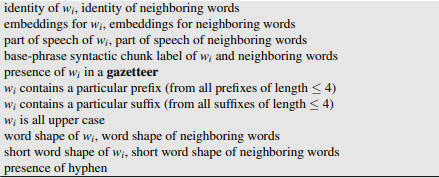
\includegraphics[scale=1]{figures/features.png}
\caption{Set of features found in Speech and Language Processing by \cite{reference1} pp. 4. for named entity recognition}
\label{fig:feature_set}
\end{figure}

From \citet{many_features} we can see the how effective many different features are on the performance of named entity recognition models. Some of the features that performed well in the paper such as suffixes and prefixes most likely won't improve the performance of our models due to objects not commonly having prefixes and suffixes. However features such as sub-tokens could be adapted to help identify units of size. The paper also goes into depth about different forms of clustering and how they can be used to help inform the model. Clustering is useful as its allows better generalisation to previously unseen words, as they can be assigned to a cluster of semantically similar words and then classified using the clusters information \citep{phrasecluster}.

\citet{refeatures} discusses the important of features in a relationship extraction task. It lays out 5 important features: the entities themselves, the types of the two entities, word sequence between the entities, number of words between the entities, and then path in the parse tree containing the two entities. For our project the types of the two entities is irrelevent as we will only be classifying sentences containing an object and a size entity.

\subsection{Preprocessing}
Due to the nature of the task, preprocessing the data may actually be detrimental to results. For example when attempting to classify a relationship between two entities it is likely that the only words between them will be stop words. Removing them in preprocessing actually may hinder the performance of the model as it will have less contextual information on which to make its classification. However this project will test the effectiveness of stop-word removal as well as lemmatisation on the performance of the models. Stemming has been left out as it will be used as a feature rather than a preproccessing technique. This is due to the similarity between lemmatisation and stemming, and wanting to test the effects stemming has as a feature.

\subsection{Labelling Data}
Once the raw text data has been acquired from our data source we will need to process and label it. The labelling process will be made easier by the creation of a labelling tool that will allow us to label entities using the BIO scheme as well as labelling the entities as having relationships or not. To properly evaluate the performance of the models a minimum number of labelled examples are needed for both sizes, objects, and relationships.  Named entity recognition has been shown to perform at expert levels with less than 100 labelled examples \citep{not_many_training_ner}, so the minimum requirement for our project will be set at 100. Relationship extraction... \\ ... \\ ... \\ ... \\ ...

\section{Programming Languages}
Despite the faster run time of Java and existence of the StanfordNLP library, for machine learning and data science, Python has the advantage. There are a significant number of libraries that will allow the implementation of this project to be much more efficient. Also despite Python running more slowly, once the models are trained the processing time of classifying a token or relationship is small enough that it will not be an issue.

\section{Datasets}
The most readily available dataset that is likely to contain information on object size would be Wikipedia. English Wikipedia can be downloaded into an xml file of just over 60GB. Due to the nature of Wikipedia and the type of information it contains it is a good candidate for our primary text dataset. As it is used for educational purposes, sentences describing objects should be more common than in other text datasets.

Another dataset that could be used to improve the performance of named entity recognition is Wordnet. Wordnet is a large lexical database of English and could be used as a gazetteer to identify entities that are objects. Wordnet will also allow the identification of multiple references to the same object as it lists alternative words for the same noun object.

\section{Databases}
The database for this project will be relatively simple and can be created using SQL, specifically MySQL it can be easily intergrated with Python. Database design guidelines explain the importance of normalising the tables to ensure that information is not stored multiple times. In the case of this project all we need to store is a reference to an object,a list of found sizes, and a link back to where each relationship was found, which is why we prefer this method over a NoSQL approach.

This is the database to store the results of our information extraction. We must also use a database to store the training data for the machine learning models. These will not need a relational database structure as all information can be contained in one row but due to the results being stored in an SQL database it makes sense for all data to be stored in the same place.

\section{Evaluation}
Dividing the labelled dataset intended for training the models into a training and testing dataset will allow us to test our models on a dataset in which we know the correct classifications. Dividing up the dataset can be done randomly and repeated a number of times to generate and average performance for each model, allowing us to get a better idea of the general performance. The metrics we will use to measure performace are precision, recall, and F1 score. The testing will test different types of model as well as how effective different features are in informing the models' classifcations.

\chapter{Methodology}
\section{Design}
Although the primary objective of the project is to generate a machine learning model that is able to detect related objects and sizes in text, there are steps that have be taken in order to get stage where we can generate and test such a model. Along with this the project also includes steps on improving the model's performance by feeding corrected low confidence classifications back into the training data. See Figure~\ref{fig:model_flow} below for an overview. \newpage

\begin{figure}[!htbp]
\centering
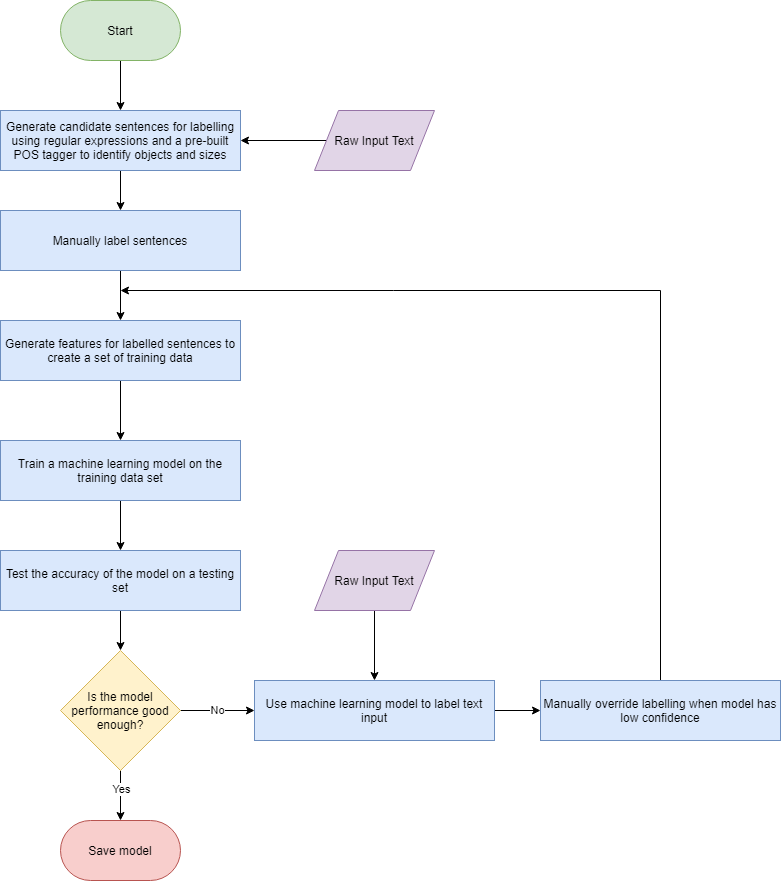
\includegraphics[scale=0.6]{figures/ModelFlowDiagram.png}
\caption{Flow diagram to show the process of generating and iteratively improving the model}
\label{fig:model_flow}
\end{figure}
\newpage

Working from this design we can break down the functions needing to be written and establish what functionality each will have to implement. 

\begin{itemize}
\item Convert raw text input into a workable format for labelling and feature generation \\
This will be the process of sentence tokenisation, breaking down the input text into single line sentences. This code will also use version 1 of the named entity recognition model to only keep sentences that it percieves to contain either an object, a size, or both.
\item Manually label the entities in the sentences and label the sentences as containing a relationship or not \\
This function will allow us to more easily label the training data. It will present each sentence one by one and take keyboard inputs to label the words within the sentence as well as the relationship.
\item Generate the features from the labelled sentences \\
This will be its own function as it is important that it is easy to switch between different feature sets for testing the models. This will take the labelled sentences as an input and output a list of features class tuples where features is a dictionary.
\item Train the models \\
Use the training data to train the models and save them as pickle files to be loaded in later.
\item Test the models \\
Test the models on a some unseen text data and recording the results for later analysis.
\end{itemize}

\subsection{Preprocessing}
Stop-word removal and lemmatisation will be performed on the data before the generation of features but after the manual labelling process. This is to increase the accuracy of manually labelling as the text will be more readable and more easily understood by humans before preprocessing.  \\ ... \\ ... \\ ... \\ Is this implementation?

\subsection{Model Design}
The design of the models comes down to the features being used to inform the classifier and the classifier itself. The features inform the classifer as to the context of the word or relationship that it has been asked to classify.

\subsubsection{Features}

The full lists of features is given in Table~\ref{tab:ner_features} and Table~\ref{tab:re_features}. All of the features will be implemented into the feature generation script and different combinations of the features will be tested against one another to optimise the performance of the models.

\begin{table}[h]
\centering
\caption{Features for named entity recognition}
\label{tab:ner_features}
\resizebox{\columnwidth}{!}{%
\begin{tabular}{|l|l|l|}
\hline
\textbf{Feature}            & \multicolumn{1}{c|}{\textbf{Description}}                                     & \multicolumn{1}{c|}{\textbf{Example}} \\ \hline
Token/word in lowercase     & The token or word to be labelled                                              & “cars"                                \\ \hline
Stemmed token               & Shortened form of the token                                                   & “car"                                 \\ \hline
Shape                       & The shape of the token how it appeared                                        & “Xxxx"                                \\ \hline
Part of speech tag          & The part of speech identified by a PoS tagger                                 & “noun"                                \\ \hline
Previous 3 tokens           & The 3 tokens to come previously in the text, blank if no more words before it & “",“two", “red"                       \\ \hline
Previous 3 token labels     & The labels given by the model the previous 3 tokens                           & “",“o",“o"                            \\ \hline
Next 3 tokens               & The 3 token to come next in the text, blank of no more words after            & “went",“down",“the"                   \\ \hline
Contains numbers            & Does the token contain numerical characters?                                  & “False"                               \\ \hline
Contains a unit of size     & Does the token contain a unit of size from a predefined list of units?        & “False"                               \\ \hline
Sub-tokens                    & If the token contains numbers and letters, seperate them into seperate tokens  & “3",“m"                                \\ \hline
\end{tabular}%
}
\end{table}

\begin{table}[h]
\centering
\caption{Features for relationship extraction}
\label{tab:re_features}
\resizebox{\columnwidth}{!}{%
\begin{tabular}{|l|l|l|}
\hline
\textbf{Feature}            & \multicolumn{1}{c|}{\textbf{Description}}                                     & \multicolumn{1}{c|}{\textbf{Example}} \\ \hline
Object entity     & The object entity in the sentence                                              & “car"                                \\ \hline
Size entity               & The size entity in the sentence                                                   & “3m"                                 \\ \hline
Words between entities   & Bag of words of all words between the two entities                  & “is",“about"                        \\ \hline
Number of words between entities   & Count of the number of words between the entities   & 2                                      \\ \hline
Presence of verb between entities    & Are any of the words between the entities a verb?    & “True"                             \\ \hline
Order of appearance        & Which entity appeared in the sentence first                        & “object"                                \\ \hline
\end{tabular}%
}
\end{table}

\subsubsection{Models}

The models are implementations of models from the {P}ython library scikit-learn \citep{scikit-learn}. Sci-kit learn provides a variety of models and by using the library we were able to implement different models and compare how they each performed on the test dataset. The models implemented are:

\begin{itemize}
\item Multinomial Naive Bayes \\
Naive Bayes model for discrete features. Has been used in text classification and has been shown to have results comparing to those of SVMs \citep{MNB}.
\item Bernoulli Naive Bayes \\
Naive Bayes model for discrete features very similar to multinomial naive bayes, however it differs in that it is designed for binary features. This model is being included as some of the features will be binary and this model could help inform the combined voting model. 
\item Logistic Regression \\
Implements regularized logistic regression.
\item Stochastic Gradient Descent \\
A standard stochastic gradient descent model, implements a regularised linear model with stochastic gradient descent.
\item Support Vector \\
A linear support vector that implements its linear classifier from libsvm \citep{libsvm}.
\item Linear Support Vector \\
A linear support vector that implements its linear classifier from liblinear \citep{liblinear} meaning that it is more suited for large datasets than the support vector model.
\item Nu-Support Vector \\
A variation on the support vector model that allows control over the number of support vectors. Will be used to test to see the effects that the number of support vectors have on the performance of the support vector models.
\item Combined Voting \\
The combined voting model will use a set of the above models to each classify the input, it will classify the input by majority vote. This aims to reduce the variance in the performance of the models. If there is an anomalous result that one of the models would have missclassified then the other models will override the vote and will correct the classification.
\end{itemize}

\section{Implementation}

\subsection{Generating the labelled data}

As outlined earlier there are a number of steps between the raw input data and the labelled features. One of the steps that could potentially be very time consuming when implementating a project of this size is labelling training data. To reduce the amount of time spent on labelling the data for this project we developed a labelling tool that allowed us to more quickly label entities and relationships. It works by displaying each candidate sentence to the user one at a time. An input of “q” means that the sentence does not contain an entity or relationship, else you would either label the entities using the BIO scheme, or label the sentence as having a relationship, depending on what you are labelling the data for.

\begin{figure}[!htbp]
\centering
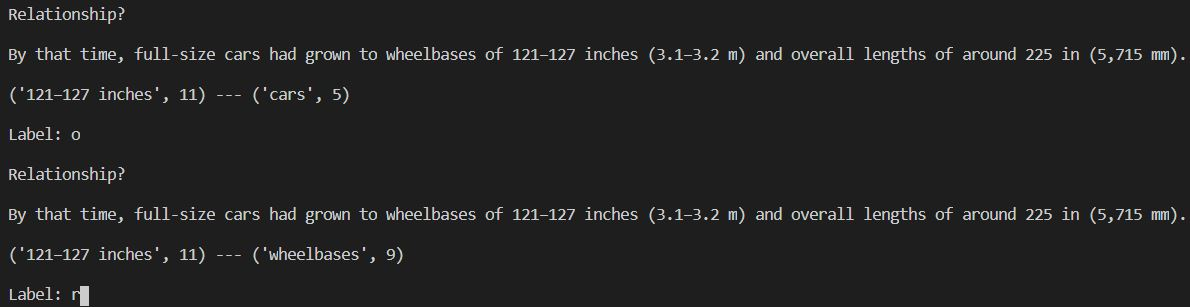
\includegraphics[scale=0.5]{images/relationship_labelling_2.jpg}
\caption{Screenshot showing the process of labelling relationships}
\label{img:relationship_labelling}
\end{figure}

Having to process and label a large number of sentences is still very time consuming, so again to speed this up we created a basic “version 1” named entity recognition model. This model identified “candidate sentences”. These are sentences that should have a higher likelihood of containing entities. The version 1 model uses regular expressions to identify sentences that contain a unit of size in them. It also uses nltk's built in part-of-speech tagger to identify nouns along with Wordnet, although accuracy in identifying candidate sentences is practically identical whether you also use Wordnet or not.

\subsection{Generating the features}
Once the data has been labelled we need to generate the features to inform the models as to the context of each classification. To do this for named entity recognition we use the sentence the token was found in, along with the labels for each token. Then using the nltk library for stemming and part of speech tagging, along with a few custom written functions for getting the token shape or the previous tokens etc, we generate a dictionary of features that can then be written to a file or added to a list of training data, along with its class label.

The process is similar for relationship extraction. In this case to generate the features we use the sentence the two types of entity were found in, along with the positions of those entities in the sentence. This is so that we can generate features such as the order that they appeared in, as well as being able to get all the words between them. Once these are generated, again we write the dictionary to a file or list with its class label.

\subsection{Training and testing the models}
The labelled features are loaded in using pickle as a list of tuples containing feature dictionaries and a class label. They are then are split into a training and testing set. When testing the average performance of the models over different training data the labelled features dataset will be randomly sorted before splitting. The split of the data is 90\% for training and 10\% for testing. The models are then successively trained on the training dataset as well as combined into the voting model, before they are all tested.

\subsection{Creating the database}
The database consists of two tables: one for storing the objects and their average size from all references, and another for storing the references found in the text to the entities and their sizes. The second table is used to calculate the average size of each object from all the various references to them found in the text. The table to store the references also stores the sentence in which the relationship was found and this is helpful when later trying to analyse the performance of the models.

\begin{figure}[!htbp]
\centering
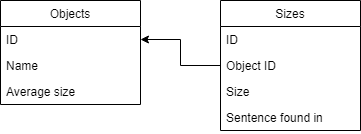
\includegraphics[scale=0.7]{figures/DatabaseDiagram.png}
\caption{Diagram to show database tables and their relations}
\label{fig:model_flow}
\end{figure}

\subsection{Extracting objects and sizes from text}
Once the models have been generated they are saved as pickle files. They can then be loaded into another Python script and used to classify incoming text inputs. The implentation of this part is very similar to the implementation of the version 1 model which was used to identify candidate sentences for labelling. The input text is broken down into sentences and run through the named entity recognition model, if both an object and size entity exist in the sentence then it is run through the relationship extraction model. If the entities are classified as being related the the database is searched to see if the object has been found before, if not the a new record is added to the objects table, else a new reference will be added in the references table and the average size updated.


\section{Testing}

All four parts of main functionality from generating the training data through to training and testing the models was tested thoroughly. Each part was tested on various inputs and edge cases to ensure that all variations of input will result in a correct output. Full tables of all tests can be found in the appendix.

\chapter{Results}

All the subsequent tests were completed on the same training and testing datasets, the only variance between them was the set of features used to inform the models, and the type of model making the classification.

\section{Named Entity Recognition}

\begin{longtable}[c]{|l|c|c|c|c|}
\caption{The features within each feature set}
\label{tab:ner_features_sets}\\
\hline
\textbf{Feature}        & \multicolumn{1}{l|}{\textbf{Set 1}} & \multicolumn{1}{l|}{\textbf{Set 2}} & \multicolumn{1}{l|}{\textbf{Set 3}} & \multicolumn{1}{l|}{\textbf{Set 4}} \\ \hline
\endfirsthead
%
\endhead
%
Token/word in lowercase & \textbf{X}                          & \textbf{X}                          & \textbf{X}                          & \textbf{X}                          \\ \hline
Stemmed token           & \textbf{X}                          & \multicolumn{1}{l|}{}               & \textbf{X}                          & \textbf{X}                          \\ \hline
Shape                   & \textbf{X}                          & \textbf{X}                          & \textbf{X}                          & \textbf{X}                          \\ \hline
Part of speech tag      & \textbf{X}                          & \textbf{X}                          & \textbf{X}                          & \textbf{X}                          \\ \hline
Previous 3 tokens       & \textbf{X}                          & \textbf{X}                          & \multicolumn{1}{l|}{}               & \textbf{X}                          \\ \hline
Previous 3 token labels & \textbf{X}                          & \textbf{X}                          & \multicolumn{1}{l|}{}               & \textbf{X}                          \\ \hline
Next 3 tokens           & \textbf{X}                          & \textbf{X}                          & \multicolumn{1}{l|}{}               & \textbf{X}                          \\ \hline
Contains numbers        & \textbf{X}                          & \textbf{X}                          & \textbf{X}                          & \multicolumn{1}{l|}{}               \\ \hline
Contains a unit of size & \textbf{X}                          & \textbf{X}                          & \textbf{X}                          & \multicolumn{1}{l|}{}               \\ \hline
Sub-tokens              & \textbf{X}                          & \textbf{X}                          & \textbf{X}                          & \multicolumn{1}{l|}{}               \\ \hline
\end{longtable}

All of these features sets were tested on each model both with preprocessing and without. Feature sets 1 - 4 have been tested both with and without preprecessing applied.

\begin{longtable}{|l|l|l|l|l|}
\caption{Models performance on feature set 1 with preprocessing for named entity recognition}
\label{tab:ner_feature_set_1}\\
\hline
\textbf{Model}          & \multicolumn{1}{c|}{\textbf{Precision}} & \multicolumn{1}{c|}{\textbf{Recall}} & \textbf{F1}  \\ \hline
\endfirsthead
%
\endhead
%
Multinomial Naive Bayes & 0.66  &  0.70   &  0.63   \\ \hline
Bernoulli Naive Bayes       & 0.27 & 0.49 & 0.34   \\ \hline
Logistic Regression         & 0.79 & 0.73 & 0.69   \\ \hline
Stochastic Gradient Descent & 0.81 & 0.76 & 0.76   \\ \hline
Support Vector              & 0.14 & 0.38 & 0.21  \\ \hline
Linear Support Vector       & 0.84 & 0.81 & 0.82  \\ \hline
Combined Voting             & 0.82 & 0.76 & 0.72  \\ \hline
\end{longtable}

\begin{longtable}{|l|l|l|l|l|}
\caption{Models performance on feature set 2 with preprocessing for named entity recognition}
\label{tab:ner_feature_set_2}\\
\hline
\textbf{Model}          & \multicolumn{1}{c|}{\textbf{Precision}} & \multicolumn{1}{c|}{\textbf{Recall}} & \textbf{F1} \\ \hline
\endfirsthead
%
\endhead
%
Multinomial Naive Bayes &  0.59  & 0.70  & 0.62 \\ \hline
Bernoulli Naive Bayes       & 0.56 & 0.62 & 0.53   \\ \hline
Logistic Regression         & 0.79 & 0.78 & 0.74  \\ \hline
Stochastic Gradient Descent & 0.84 & 0.81 & 0.81  \\ \hline
Support Vector              & 0.19 & 0.43 & 0.26  \\ \hline
Linear Support Vector       & 0.85 & 0.84 & 0.84  \\ \hline
Combined Voting             & 0.79 & 0.78 & 0.74  \\ \hline
\end{longtable}

\begin{longtable}{|l|l|l|l|l|}
\caption{Models performance on feature set 3 with preprocessing for named entity recognition}
\label{tab:ner_feature_set_3}\\
\hline
\textbf{Model}          & \multicolumn{1}{c|}{\textbf{Precision}} & \multicolumn{1}{c|}{\textbf{Recall}} & \textbf{F1} \\ \hline
\endfirsthead
%
\endhead
%
Multinomial Naive Bayes &  0.48  & 0.59  & 0.50   \\ \hline
Bernoulli Naive Bayes       & 0.48 & 0.59 & 0.50   \\ \hline
Logistic Regression         & 0.53 & 0.62 & 0.54  \\ \hline
Stochastic Gradient Descent & 0.77 & 0.65 & 0.60  \\ \hline
Support Vector              &  0.11 & 0.32 & 0.16  \\ \hline
Linear Support Vector       & 0.53 & 0.65 & 0.57  \\ \hline
Combined Voting             & 0.53 & 0.62 & 0.54   \\ \hline
\end{longtable}

\begin{longtable}{|l|l|l|l|l|}
\caption{Models performance on feature set 4 with preprocessing for named entity recognition}
\label{tab:ner_feature_set_4}\\
\hline
\textbf{Model}          & \multicolumn{1}{c|}{\textbf{Precision}} & \multicolumn{1}{c|}{\textbf{Recall}} & \textbf{F1} \\ \hline
\endfirsthead
%
\endhead
%
Multinomial Naive Bayes &  0.77  & 0.70  & 0.65  \\ \hline
Bernoulli Naive Bayes       & 0.27 & 0.51 & 0.35   \\ \hline
Logistic Regression         & 0.82 & 0.78 & 0.76   \\ \hline
Stochastic Gradient Descent & 0.80 & 0.73 & 0.73   \\ \hline
Support Vector              & 0.21 & 0.46 & 0.29   \\ \hline
Linear Support Vector       & 0.76 & 0.76 & 0.74   \\ \hline
Combined Voting             & 0.82 & 0.78 & 0.76   \\ \hline
\end{longtable}

\begin{longtable}{|l|l|l|l|l|}
\caption{Models performance on feature set 1 without preprocessing for named entity recognition}
\label{tab:ner_feature_set_5}\\
\hline
\textbf{Model}          & \multicolumn{1}{c|}{\textbf{Precision}} & \multicolumn{1}{c|}{\textbf{Recall}} & \textbf{F1} \\ \hline
\endfirsthead
%
\endhead
%
Multinomial Naive Bayes &  0.76  & 0.83  & 0.79  \\ \hline
Bernoulli Naive Bayes       & 0.69 & 0.79 & 0.72   \\ \hline
Logistic Regression         & 0.79 & 0.85 & 0.82   \\ \hline
Stochastic Gradient Descent & 0.83 & 0.83 & 0.82   \\ \hline
Support Vector              & 0.51 & 0.71 & 0.59   \\ \hline
Linear Support Vector       & 0.82 & 0.85 & 0.83   \\ \hline
Combined Voting             & 0.77 & 0.83 & 0.80   \\ \hline
\end{longtable}

\begin{longtable}{|l|l|l|l|l|}
\caption{Models performance on feature set 2 without preprocessing for named entity recognition}
\label{tab:ner_feature_set_6}\\
\hline
\textbf{Model}          & \multicolumn{1}{c|}{\textbf{Precision}} & \multicolumn{1}{c|}{\textbf{Recall}} & \textbf{F1} \\ \hline
\endfirsthead
%
\endhead
%
Multinomial Naive Bayes &  0.80  & 0.86  & 0.82       \\ \hline
Bernoulli Naive Bayes       & 0.57 & 0.67 & 0.57   \\ \hline
Logistic Regression         & 0.78 & 0.83 & 0.79   \\ \hline
Stochastic Gradient Descent & 0.86 & 0.83 & 0.84   \\ \hline
Support Vector              & 0.35 & 0.59 & 0.44   \\ \hline
Linear Support Vector       & 0.87 & 0.86 & 0.86   \\ \hline
Combined Voting             & 0.78 & 0.85 & 0.80   \\ \hline
\end{longtable}

\begin{longtable}{|l|l|l|l|l|}
\caption{Models performance on feature set 3 without preprocessing for named entity recognition}
\label{tab:ner_feature_set_7}\\
\hline
\textbf{Model}          & \multicolumn{1}{c|}{\textbf{Precision}} & \multicolumn{1}{c|}{\textbf{Recall}} & \textbf{F1} \\ \hline
\endfirsthead
%
\endhead
%
Multinomial Naive Bayes &  0.90  & 0.89  & 0.89      \\ \hline
Bernoulli Naive Bayes       & 0.76 & 0.86 & 0.81   \\ \hline
Logistic Regression         & 0.89 & 0.91 & 0.90  \\ \hline
Stochastic Gradient Descent & 0.91 & 0.89 & 0.90   \\ \hline
Support Vector              & 0.62 & 0.79 & 0.69   \\ \hline
Linear Support Vector       & 0.92 & 0.92 & 0.92   \\ \hline
Combined Voting             & 0.89 & 0.91 & 0.90   \\ \hline
\end{longtable}

\begin{longtable}{|l|l|l|l|l|}
\caption{Models performance on feature set 4 without preprocessing for named entity recognition}
\label{tab:ner_feature_set_8}\\
\hline
\textbf{Model}          & \multicolumn{1}{c|}{\textbf{Precision}} & \multicolumn{1}{c|}{\textbf{Recall}} & \textbf{F1} \\ \hline
\endfirsthead
%
\endhead
%
Multinomial Naive Bayes &  0.66  & 0.76  & 0.70     \\ \hline
Bernoulli Naive Bayes       & 0.62 & 0.73 & 0.64  \\ \hline
Logistic Regression         & 0.80 & 0.83 & 0.79  \\ \hline
Stochastic Gradient Descent & 0.86 & 0.83 & 0.83  \\ \hline
Support Vector              & 0.46 & 0.68 & 0.55  \\ \hline
Linear Support Vector       & 0.90 & 0.89 & 0.87  \\ \hline
Combined Voting             & 0.82 & 0.86 & 0.83  \\ \hline
\end{longtable}

\begin{longtable}[c]{|l|l|l|}
\caption{Preprocessing F1 averages for all models on different feature sets}
\label{tab:ner_preprocessing}\\
\hline
\textbf{\begin{tabular}[c]{@{}l@{}}Feature \\ Set\end{tabular}} & \textbf{Preprocessing} & \textbf{\begin{tabular}[c]{@{}l@{}}No\\ Preprocessing\end{tabular}} \\ \hline
\endfirsthead
%
\endhead
%
1 & 0.60 & 0.77 \\ \hline
2 & 0.65 & 0.73 \\ \hline
3 & 0.49 & 0.86 \\ \hline
4 & 0.61 & 0.74 \\ \hline
\end{longtable}

\section{Relationship Extraction}

These tests were performed on labelled entity information not from sentences labelled by the named entity recognition model. Due to the small number of features used, only one set was tested.

\begin{longtable}{|l|l|l|l|l|}
\caption{Models performance with preprocessing for relationship extraction}
\label{tab:re_feature_set_1}\\
\hline
\textbf{Model}          & \multicolumn{1}{c|}{\textbf{Precision}} & \multicolumn{1}{c|}{\textbf{Recall}} & \textbf{F1} \\ \hline
\endfirsthead
%
\endhead
%
Multinomial Naive Bayes &  0.66  & 0.69  & 0.66  \\ \hline
Bernoulli Naive Bayes       & 0.83 & 0.77 & 0.72  \\ \hline
Logistic Regression         & 0.83 & 0.77 & 0.72  \\ \hline
Stochastic Gradient Descent & 0.48 & 0.69 & 0.57  \\ \hline
Support Vector              & 0.48 & 0.69 & 0.57  \\ \hline
Linear Support Vector       & 0.66 & 0.69 & 0.66  \\ \hline
Combined Voting             & 0.83 & 0.77 & 0.72  \\ \hline
\end{longtable}

\begin{longtable}{|l|l|l|l|l|}
\caption{Models performance without preprocessing for relationship extraction}
\label{tab:re_feature_set_2}\\
\hline
\textbf{Model}          & \multicolumn{1}{c|}{\textbf{Precision}} & \multicolumn{1}{c|}{\textbf{Recall}} & \textbf{F1} \\ \hline
\endfirsthead
%
\endhead
%
Multinomial Naive Bayes &  &  &   \\ \hline
Bernoulli Naive Bayes       &  &  &   \\ \hline
Logistic Regression         &  &  &   \\ \hline
Stochastic Gradient Descent &  &  &   \\ \hline
Support Vector              &  &  &   \\ \hline
Linear Support Vector      &  &  &   \\ \hline
Combined Voting             &  &  &   \\ \hline
\end{longtable}

\section{Named Entity Recognition and Relationship Extraction}

Testing first the named entity recognition model and then feeding those classifications into the relationship extraction model to fully test the entire information extraction system.

\begin{longtable}{|l|l|l|l|l|}
\caption{Models performance on feature set 1}
\label{tab:ner_re_feature_set_1}\\
\hline
\textbf{Model}          & \multicolumn{1}{c|}{\textbf{Precision}} & \multicolumn{1}{c|}{\textbf{Recall}} & \textbf{F1} & \textbf{F1 Variance} \\ \hline
\endfirsthead
%
\endhead
%
Multinomial Naive Bayes & \multicolumn{1}{c|}{}                   & \multicolumn{1}{c|}{}                &             &                      \\ \hline
Bernoulli Naive Bayes       &  &  &  &  \\ \hline
Logistic Regression         &  &  &  &  \\ \hline
Stochastic Gradient Descent &  &  &  &  \\ \hline
Support Vector              &  &  &  &  \\ \hline
Linear Support Vector       &  &  &  &  \\ \hline
Nu-Support Vector (0.3)     &  &  &  &  \\ \hline
Nu-Support Vector (0.5)     &  &  &  &  \\ \hline
Nu-Support Vector (0.7)     &  &  &  &  \\ \hline
Combined Voting             &  &  &  &  \\ \hline
\end{longtable}

\begin{longtable}{|l|l|l|l|l|}
\caption{Models performance on feature set 2}
\label{tab:ner_re_feature_set_2}\\
\hline
\textbf{Model}          & \multicolumn{1}{c|}{\textbf{Precision}} & \multicolumn{1}{c|}{\textbf{Recall}} & \textbf{F1} & \textbf{F1 Variance} \\ \hline
\endfirsthead
%
\endhead
%
Multinomial Naive Bayes & \multicolumn{1}{c|}{}                   & \multicolumn{1}{c|}{}                &             &                      \\ \hline
Bernoulli Naive Bayes       &  &  &  &  \\ \hline
Logistic Regression         &  &  &  &  \\ \hline
Stochastic Gradient Descent &  &  &  &  \\ \hline
Support Vector              &  &  &  &  \\ \hline
Linear Support Vector       &  &  &  &  \\ \hline
Nu-Support Vector (0.3)     &  &  &  &  \\ \hline
Nu-Support Vector (0.5)     &  &  &  &  \\ \hline
Nu-Support Vector (0.7)     &  &  &  &  \\ \hline
Combined Voting             &  &  &  &  \\ \hline
\end{longtable}

\begin{longtable}[c]{|l|l|l|l|l|}
\caption{Preprocessing F1 averages for all models on different feature sets}
\label{tab:ner_re_preprocessing}\\
\hline
\textbf{\begin{tabular}[c]{@{}l@{}}Feature \\ Set\end{tabular}} & \multicolumn{1}{c|}{\textbf{None}} & \multicolumn{1}{c|}{\textbf{S}} & \multicolumn{1}{c|}{\textbf{L}} & \multicolumn{1}{c|}{\textbf{S, L}} \\ \hline
\endfirsthead
%
\endhead
%
1                                                               & \multicolumn{1}{c|}{}              & \multicolumn{1}{c|}{}           &                                 &                                    \\ \hline
2                                                               &                                    &                                 &                                 &                                    \\ \hline
3                                                               &                                    &                                 &                                 &                                    \\ \hline
\end{longtable}

\chapter{Discussion}

\section{Goals achieved}


\section{Future Improvements}
With more time and computational power a wider variety of machine learning models could be tested to see how they perform. Sci-kit learn from which the models implemented are taken, provides more models that were not implemented due to the scope of the project. There could also be investigation into other libraries or custom implementations of models.

Again, given more time, the scope of this project could have been expanded in terms of the different features tested and the size of the training dataset. These likely would have a greater effect on the performance than a different type of model. These could be achieved by further analysis of the target text datasets to help indicate what features could be informative in making a classification, as well as further reading around the topic into existing named enitity recognition and relationship extraction projects.

One of the features tested was the class label of previous tokens. This could be expanded to also include class labels on the next tokens in the sentence. To do this the model needs to perform two passes over the sentence, the first in which it does not take into account the labels of other tokens, and the second in which it does.

\chapter{Conclusion}



% -------------------------------------------------------------------
% Bibliography
% -------------------------------------------------------------------
\addcontentsline{toc}{chapter}{Bibliography}
\bibliographystyle{agsm} 
\bibliography{mybibliography} 


% -------------------------------------------------------------------
% Appendices
% -------------------------------------------------------------------

\begin{appendices}
\chapter{Testing}

\subsection{Getting candidate sentences}
\begin{longtable}[c]{|l|l|l|l|}
\caption{Tests performed on the generation of candidate sentences for the labelled training data}
\label{tab:candidate_tests}\\
\hline
\textbf{Test} & \textbf{Input} & \textbf{\begin{tabular}[c]{@{}l@{}}Expected\\ Output\end{tabular}} & \textbf{Pass/Fail} \\ \hline
\endfirsthead
%
\endhead
%
Iterating through all sentences & \begin{tabular}[c]{@{}l@{}}Text containing multiple\\ sentences per line\end{tabular} & \begin{tabular}[c]{@{}l@{}}Iterates over each\\ sentence on each line\end{tabular} & Pass \\ \hline
\begin{tabular}[c]{@{}l@{}}Outputs candidate sentences\\ to file\end{tabular} & - & \begin{tabular}[c]{@{}l@{}}candidate sentences\\ text file\end{tabular} & Pass \\ \hline
Wordnet detects noun & \begin{tabular}[c]{@{}l@{}}Sentence with no Wordnet\\ noun\\ \\ Sentence with Wordnet noun\end{tabular} & \begin{tabular}[c]{@{}l@{}}Not candidate\\ sentence\\ \\ Candidate sentence\end{tabular} & \begin{tabular}[c]{@{}l@{}}Pass\\ \\ \\ Pass\end{tabular} \\ \hline
\begin{tabular}[c]{@{}l@{}}Part of speech tagger detects\\ noun\end{tabular} & \begin{tabular}[c]{@{}l@{}}Sentence not containing\\ noun\\ \\ Sentence containing\\ noun\end{tabular} & \begin{tabular}[c]{@{}l@{}}Not candidate\\ sentence\\ \\ Candidate sentence\end{tabular} & \begin{tabular}[c]{@{}l@{}}Pass\\ \\ \\ Pass\end{tabular} \\ \hline
Regex detects size & \begin{tabular}[c]{@{}l@{}}Sentence with no unit of size\\ \\ \\ Sentence with unit of size\end{tabular} & \begin{tabular}[c]{@{}l@{}}Not candidate\\ sentence\\ \\ Candidate sentence\end{tabular} & \begin{tabular}[c]{@{}l@{}}Pass\\ \\ \\ Pass\end{tabular} \\ \hline
\end{longtable}

\subsection{Labelling sentences}
\begin{longtable}[c]{|l|l|l|l|}
\caption{Tests performed on the labelling tool for generating labelled training data}
\label{tab:labelling_tests}\\
\hline
\textbf{Test} & \textbf{Input} & \textbf{\begin{tabular}[c]{@{}l@{}}Expected\\ Output\end{tabular}} & \textbf{Pass/Fail} \\ \hline
\endfirsthead
%
\endhead
%
Iterating through all sentences & \begin{tabular}[c]{@{}l@{}}Text containing multiple\\ sentences per line\end{tabular} & \begin{tabular}[c]{@{}l@{}}Iterates over each\\ sentence on each line\end{tabular} & Pass \\ \hline
Labelling different entities & \begin{tabular}[c]{@{}l@{}}Sentence containing objects,\\ sizes, and non-entities\end{tabular} & \begin{tabular}[c]{@{}l@{}}Labels entities using\\ BIO scheme\end{tabular} & Pass \\ \hline
Labelling relationships & \begin{tabular}[c]{@{}l@{}}Sentence containing\\ relationship\\ \\ Sentence not containing\\ relationship\end{tabular} & \begin{tabular}[c]{@{}l@{}}Labels sentence as\\ "relationship"\\ \\ Labels sentence as\\ "o"\end{tabular} & \begin{tabular}[c]{@{}l@{}}Pass\\ \\ \\ Pass\end{tabular} \\ \hline
\begin{tabular}[c]{@{}l@{}}Outputting labelled sentences\\ to a file\end{tabular} & - & \begin{tabular}[c]{@{}l@{}}labelled sentences\\ text file\end{tabular} & Pass \\ \hline
\begin{tabular}[c]{@{}l@{}}Skipping relationship labelling\\ of not at least one of each\\ entity\end{tabular} & \begin{tabular}[c]{@{}l@{}}Text only containing an object\\ \\ Text only containing a size\\ \\ Text containing no entities\end{tabular} & \begin{tabular}[c]{@{}l@{}}Labels as "o"\\ \\ Labels as "o"\\ \\ Labels as "o"\end{tabular} & \begin{tabular}[c]{@{}l@{}}Pass\\ \\ Pass\\ \\ Pass\end{tabular} \\ \hline
Label all as "o" input & \begin{tabular}[c]{@{}l@{}}Inputting "q" at start of\\ sentence\end{tabular} & \begin{tabular}[c]{@{}l@{}}Labels sentence as \\ "o"\end{tabular} & Pass \\ \hline
\begin{tabular}[c]{@{}l@{}}Label rest of sentence as "o"\\ input\end{tabular} & \begin{tabular}[c]{@{}l@{}}Inputting "q" midway through\\ sentence\end{tabular} & \begin{tabular}[c]{@{}l@{}}Labels first half as\\ input, second has as\\ "o"\end{tabular} & Pass \\ \hline
\end{longtable}

\subsection{Generating features}
\begin{longtable}[c]{|l|l|l|l|}
\caption{Tests performed on the generation of different features for the named entity recognition models}
\label{tab:ner_features_tests}\\
\hline
\textbf{Test} & \textbf{Input} & \textbf{\begin{tabular}[c]{@{}l@{}}Expected\\ Output\end{tabular}} & \textbf{Pass/Fail} \\ \hline
\endfirsthead
%
\endhead
%
Token & "token" & "token" & Pass \\ \hline
Stemmed token & \begin{tabular}[c]{@{}l@{}}"build"\\ \\ "builds"\\ \\ "building"\\ \\ "buildings"\end{tabular} & \begin{tabular}[c]{@{}l@{}}"build"\\ \\ "build"\\ \\ "build"\\ \\ "build"\end{tabular} & \begin{tabular}[c]{@{}l@{}}Pass\\ \\ Pass\\ \\ Pass\\ \\ Pass\end{tabular} \\ \hline
Shape & \begin{tabular}[c]{@{}l@{}}"Title"\\ \\ "lower"\\ \\ "UPPER"\end{tabular} & \begin{tabular}[c]{@{}l@{}}"Xxxxx"\\ \\ "xxxxx"\\ \\ "XXXXX"\end{tabular} & \begin{tabular}[c]{@{}l@{}}Pass\\ \\ Pass\\ \\ Pass\end{tabular} \\ \hline
Part of speech tag & \begin{tabular}[c]{@{}l@{}}"saw" in sentence as noun\\ \\ "saw" in sentence as verb\end{tabular} & \begin{tabular}[c]{@{}l@{}}Tagged as noun\\ \\ Tagged as verb\end{tabular} & \begin{tabular}[c]{@{}l@{}}Pass\\ \\ Pass\end{tabular} \\ \hline
Previous 3 tokens & \begin{tabular}[c]{@{}l@{}}Token, 1st in sentence\\ \\ Token, 2nd in sentence\\ \\ \\ \\ Token, 3rd in sentence\\ \\ \\ \\ Token, 4th in sentence\end{tabular} & \begin{tabular}[c]{@{}l@{}}Three empty strings\\ \\ Two empty strings\\ and previous token\\ \\ One empty string\\ and two previous\\ tokens\\ \\ Three previous\\ tokens\end{tabular} & \begin{tabular}[c]{@{}l@{}}Pass\\ \\ Pass\\ \\ \\ \\ Pass\\ \\ \\ \\ Pass\end{tabular} \\ \hline
Next 3 tokens & \begin{tabular}[c]{@{}l@{}}Token, 4th last in sentence\\ \\ Token, 3rd last in sentence\\ \\ \\ Token, 2nd last in sentence\\ \\ \\ Token, last in sentence\end{tabular} & \begin{tabular}[c]{@{}l@{}}Next three tokens\\ \\ Next two tokens and \\ empty string\\ \\ Next token and two\\ empty strings\\ \\ Three empty strings\end{tabular} & \begin{tabular}[c]{@{}l@{}}Pass\\ \\ Pass\\ \\ \\ Pass\\ \\ \\ Pass\end{tabular} \\ \hline
\begin{tabular}[c]{@{}l@{}}Presence in Wordnet\\ as a noun\end{tabular} & \begin{tabular}[c]{@{}l@{}}Token that is noun in Wordnet\\ \\ Token that isn't noun in\\ Wordnet\end{tabular} & \begin{tabular}[c]{@{}l@{}}"True"\\ \\ "False"\end{tabular} & \begin{tabular}[c]{@{}l@{}}Pass\\ \\ Pass\end{tabular} \\ \hline
Contains numbers & \begin{tabular}[c]{@{}l@{}}"nonumbers"\\ \\ "numbers123"\end{tabular} & \begin{tabular}[c]{@{}l@{}}"False"\\ \\ "True"\end{tabular} & \begin{tabular}[c]{@{}l@{}}Pass\\ \\ Pass\end{tabular} \\ \hline
\begin{tabular}[c]{@{}l@{}}Contains a unit of\\ size\end{tabular} & \begin{tabular}[c]{@{}l@{}}"nounit"\\ \\ "cm"\end{tabular} & \begin{tabular}[c]{@{}l@{}}"False"\\ \\ "True"\end{tabular} & \begin{tabular}[c]{@{}l@{}}Pass\\ \\ Pass\end{tabular} \\ \hline
Sub-tokens & \begin{tabular}[c]{@{}l@{}}"token"\\ \\ "12cm"\end{tabular} & \begin{tabular}[c]{@{}l@{}}Empty tuple\\ \\ "12", "cm"\end{tabular} & \begin{tabular}[c]{@{}l@{}}Pass\\ \\ Pass\end{tabular} \\ \hline
\end{longtable}


\begin{longtable}[c]{|l|l|l|l|}
\caption{Tests performed on the generation of different features for the relationship extraction models}
\label{tab:re_features_tests}\\
\hline
\textbf{Test} & \textbf{Input} & \textbf{\begin{tabular}[c]{@{}l@{}}Expected\\ Output\end{tabular}} & \textbf{Pass/Fail} \\ \hline
\endfirsthead
%
\endhead
%
Object entity & \begin{tabular}[c]{@{}l@{}}Sentence with object\\ entity "Alex"\end{tabular} & "Alex" & Pass \\ \hline
Size entity & \begin{tabular}[c]{@{}l@{}}Sentence with size\\ entity "6 foot 3 inches"\end{tabular} & "6 foot 3 inches" & Pass \\ \hline
\begin{tabular}[c]{@{}l@{}}Bag of words\\ between entities\end{tabular} & \begin{tabular}[c]{@{}l@{}}No words between\\ entities\\ \\ No repeating words\\ between entities\\ \\ Repeating words between\\ entities\end{tabular} & \begin{tabular}[c]{@{}l@{}}Empty list\\ \\ \\ List of words\\ \\ \\ List of unique words\end{tabular} & \begin{tabular}[c]{@{}l@{}}Pass\\ \\ \\ Pass\\ \\ \\ Pass\end{tabular} \\ \hline
\begin{tabular}[c]{@{}l@{}}Number of words\\ between entities\end{tabular} & \begin{tabular}[c]{@{}l@{}}No words between entities\\ \\ 5 words between entities\end{tabular} & \begin{tabular}[c]{@{}l@{}}0\\ \\ 5\end{tabular} & \begin{tabular}[c]{@{}l@{}}Pass\\ \\ Pass\end{tabular} \\ \hline
\begin{tabular}[c]{@{}l@{}}Presence of verb\\ between entities\end{tabular} & \begin{tabular}[c]{@{}l@{}}No words between entities\\ \\ Non-verbs between\\ entities\\ \\ Verb between entities\end{tabular} & \begin{tabular}[c]{@{}l@{}}"False"\\ \\ "False"\\ \\ \\ "True"\end{tabular} & \begin{tabular}[c]{@{}l@{}}Pass\\ \\ Pass\\ \\ \\ Pass\end{tabular} \\ \hline
\begin{tabular}[c]{@{}l@{}}Order of\\ appearance\end{tabular} & \begin{tabular}[c]{@{}l@{}}Object appears first\\ \\ Size appears first\end{tabular} & \begin{tabular}[c]{@{}l@{}}"Object"\\ \\ "Size"\end{tabular} & \begin{tabular}[c]{@{}l@{}}Pass\\ \\ Pass\end{tabular} \\ \hline
\end{longtable}

\subsection{Training and testing models}
\begin{longtable}[c]{|l|l|l|l|}
\caption{Tests performed on the labelling tool for generating labelled training data}
\label{tab:model_tests}\\
\hline
\textbf{Test} & \textbf{Input} & \textbf{\begin{tabular}[c]{@{}l@{}}Expected\\ Output\end{tabular}} & \textbf{Pass/Fail} \\ \hline
\endfirsthead
%
\endhead
%
\begin{tabular}[c]{@{}l@{}}Split labelled features into\\ training and testing sets\end{tabular} & Labelled features dataset & \begin{tabular}[c]{@{}l@{}}Training and testing\\ datasets\end{tabular} & Pass \\ \hline
Trains models & Training data & Trained model & Pass \\ \hline
Tests models & Testing data, model & Model performance & Pass \\ \hline
\begin{tabular}[c]{@{}l@{}}Outputs models as pickle\\ files\end{tabular} & - & \begin{tabular}[c]{@{}l@{}}A pickle file for \\ each model\end{tabular} & Pass \\ \hline
\begin{tabular}[c]{@{}l@{}}Outputs model performance\\ into logfile\end{tabular} & - & Logfile & Pass \\ \hline
\end{longtable}
\end{appendices}

\end{document}
